\documentclass[xcolor=dvipsnames,10pt]{beamer}
% ********** Style prezentation **********

\usepackage{verbatim}
\usepackage{color}
\usepackage{multimedia}
\usepackage{xmpmulti}
\usepackage[absolute,overlay]{textpos} 
\usepackage{listings}
\usepackage{algorithm}
\usepackage{algorithmic}
\usepackage{amsmath}
\usepackage{pifont}
\usepackage{url}
\usepackage{pict2e}
\usepackage{flushend}
\usepackage{graphicx}
\usepackage{pgf}
\usepackage{url}
\usepackage{tikz}
\usetikzlibrary{calc}
\usetikzlibrary{shapes}
\usetikzlibrary{backgrounds}
\usepackage{pgfplots}
\usepackage{pgfplotstable}

\newcommand{\ignore}[1]{}


\lstset{ %
  language=Java,              
  basicstyle=\footnotesize
}

\pgfdeclarelayer{foreground}
\pgfdeclarelayer{background}
\pgfsetlayers{background,main,foreground}

\mode<presentation>
{
	\usetheme{Warsaw}
}
\definecolor{scarlet}{RGB}{200,0,0}
\setbeamercolor{structure}{fg=scarlet}
\addtobeamertemplate{footline}{
\begin{columns}
  \hfill
\includegraphics[height=.75cm]{unl_clear.pdf}\hspace{.5cm}
\end{columns}
\vspace{2mm}
}{\usebeamercolor[bg]{footline}\hfill\raisebox{1mm}[0mm]{\hspace{2mm}}}

\newcommand\x[1]{\ensuremath{\mathit{#1}}}
\newcommand\lrangle[1]{\ensuremath{\langle#1\rangle}}

\def\ON{\ding{52}}
\def\OF{\ding{55}}
\def~{\phantom{0}}

\setbeamertemplate{navigation symbols}{} %remove if navigation symbols are needed
\setbeamersize{text margin left=5mm, text margin right=5mm} % change margin as you wish

\author{Matthew B. Dwyer, Antonio Filieri, Jaco Geldenhuys, Mitchell Gerrard, Corina P{\u{a}}s{\u{a}}reanu, and Willem Visser}

\title[Probabilistic Program Analysis]{Probabilistic Program Analysis}
\subtitle{}


\institute{
Department of Computer Science and Engineering\\
University of Nebraska - Lincoln\\
Lincoln, Nebraska USA\\
}

\date{August 2015}

\begin{document}

\begin{frame}
	\titlepage %displays the title page

\end{frame}


\begin{frame}[fragile]
\frametitle{Your view of ``Program Analysis''}
\vfill
When you hear the term program analysis what comes to mind?
\vfill
\pause
What applications?
\vfill
What kinds of information are computed?
\vfill
What's the relationship between that information and program semantics?
\vfill
How are the analysis results computed?
\vfill
\end{frame}

\begin{frame}[fragile]
\frametitle{Program analysis to me}
\vfill
I worked at a compiler company in the 1980s; responsible for the common optimizer in a family of C compilers for embedded systems
\vfill
My Ph.D. work applied data flow analysis to check safety properties of concurrent programs 
\vfill
Co-directed a large project on software model checking (e.g., Bandera,Bogor)
\vfill
Developed symbolic execution for program equivalence checking
\vfill
Optimization of runtime monitoring for complex properties (e.g., state machines)
\vfill
Verification of high-performance computing codes (e.g., MPI, OpenMP, CUDA, pthreads)
\vfill
\end{frame}

\ignore{
\begin{frame}[fragile]
\frametitle{Program analysis to me}
\vfill
\vfill
\end{frame}
}

\begin{frame}[fragile]
\frametitle{What is a probabilistic program?}
\vfill
\pause
Classic view is due to Kozen's 1978 semantics
\begin{itemize}
\item enrich your favorite language with the ability to draw from a probability distribution, e.g., \texttt{normal(0,1)}
\end{itemize}
\vfill
\pause
Pretty much every program is probabilistic in this sense; inputs are distributed in some way
\vfill
\pause
Modern view is that probabilistic programs encode \textit{probabilistic graphical models} which capture conditional dependence between random variables
\begin{itemize}
\item further enrich language with the ability to condition the output, e.g., \texttt{observe(x>0)}
\end{itemize}
\vfill
\pause
The modern view is being driven by applications of machine learning
\begin{itemize}
\item Infering an input distribution from (enough) observed outputs amounts to 
a backward data flow analysis (Claret et al, FSE'13)
\end{itemize}
\vfill
\end{frame}

\begin{frame}[fragile]
\frametitle{What is a probabilistic program?}
\vfill
Classic view is due to Kozen's 1978 semantics
\begin{itemize}
\item \textcolor{red}{Enrich your favorite language with the ability to draw from a probability distribution, e.g., \texttt{normal(0,1)}}
\end{itemize}
\vfill
Pretty much every program is probabilistic in this sense; \textcolor{red}{inputs are distributed in some way}
\vfill
Modern view is that probabilistic programs encode \textit{probabilistic graphical models} which capture conditional dependence between random variables
\begin{itemize}
\item Further enrich language with the ability to condition the output, e.g., \texttt{observe(x>0)}
\end{itemize}
\vfill
The modern view is being driven by applications of machine learning
\begin{itemize}
\item Infering an input distribution from (enough) observed outputs amounts to 
a backward data flow analysis 
\end{itemize}
\vfill
\end{frame}

\pgfmathdeclarefunction{Gauss}{2}{%
  \pgfmathparse{1/(#2*sqrt(2*pi))*exp(-((\x-#1)^2)/(2*#2^2))}%
}

\pgfmathdeclarefunction{RightMirrorPiledGauss}{2}{%
 \pgfmathparse{x<0?0:2*Gauss(#1,#2)}%
}

\begin{frame}[fragile]
\frametitle{Imagine an input distributed according to $N(0,2)$}
\begin{tikzpicture}
\begin{axis}[xlabel=$x$, grid=major, samples=100, domain=-10:10]
\addplot[green,very thick] {Gauss(0,2)};
\end{axis}
\end{tikzpicture}
\end{frame}

\begin{frame}[fragile]
\frametitle{A trivial program}
\vfill
\begin{center}
\begin{lstlisting}
double abs(double x) {
  if (x<0) 
    return -x;
  else 
    return x;
}
\end{lstlisting}
\end{center}
\vfill
\end{frame}

\begin{frame}[fragile]
\frametitle{Here is the output distribution}
\begin{tikzpicture}
\begin{axis}[xlabel=$x$, grid=major, samples=100, domain=-10:10]
\addplot[blue,very thick] {RightMirrorPiledGauss(0,2)};
\end{axis}
\end{tikzpicture}
\end{frame}

\begin{frame}[fragile]
\frametitle{What's going on here?}
\vfill
\begin{tikzpicture}

\begin{axis}[xlabel=$x$, grid=major, samples=100, domain=-10:10]
\addplot[green,very thick] {Gauss(0,2)};
\end{axis}

\begin{pgfonlayer}{background}
\path[fill=black!10] (0,0) rectangle (3.4,5.7);
\node at (2,4) {$x<0$};  
\node at (4.8,4) {$x \ge 0$};  
\end{pgfonlayer}

\end{tikzpicture}
\vfill
Let's think in terms of a very coarse division of the input

\end{frame}

\begin{frame}[fragile]
\frametitle{What's going on here?}
\vfill
\begin{tikzpicture}

\begin{axis}[xlabel=$x$, grid=major, samples=100, domain=-10:10]
\addplot[green,very thick] {Gauss(0,2)};
\end{axis}

\begin{pgfonlayer}{background}
\path[fill=black!10] (0,0) rectangle (3.4,5.7);
\node at (2,4) {$x<0$};  
\node at (4.8,4) {\textcolor{red}{$x \ge 0$}};  
\end{pgfonlayer}

\end{tikzpicture}
\vfill
Input values $x \ge 0$ appear on the output unchanged.
\pause

Their mass in the input distribution propagates to the output.

\end{frame}

\begin{frame}[fragile]
\frametitle{What's going on here?}
\vfill
\begin{tikzpicture}

\begin{axis}[xlabel=$x$, grid=major, samples=100, domain=-10:10]
\addplot[green,very thick] {Gauss(0,2)};
\end{axis}

\begin{pgfonlayer}{background}
\path[fill=black!10] (0,0) rectangle (3.4,5.7);
\node at (2,4) {\textcolor{red}{$x<0$}};  
\node at (4.8,4) {$x \ge 0$};  
\end{pgfonlayer}

\begin{pgfonlayer}{foreground}
\path[fill] (2.47,1.65) circle [radius=0.1];
\end{pgfonlayer}

\end{tikzpicture}
\vfill
Input values $x < 0$ are transformed.

\end{frame}

\begin{frame}[fragile]
\frametitle{What's going on here?}
\vfill
\begin{tikzpicture}
\begin{axis}[xlabel=$x$, grid=major, samples=100, domain=-10:10]
\addplot[green,very thick] {Gauss(0,2)};
\end{axis}
\begin{pgfonlayer}{background}
\path[fill=black!10] (0,0) rectangle (3.4,5.7);
\node at (2,4) {\textcolor{red}{$x<0$}};  
\node at (4.8,4) {$x \ge 0$};  
\end{pgfonlayer}
\begin{pgfonlayer}{foreground}
\path[fill] (2.47,1.65) circle [radius=0.1];
\onslide<2>\draw[->] (2.47,1.65) -> (4.37,1.65);
\end{pgfonlayer}
\end{tikzpicture}
\vfill
Input values $x < 0$ are transformed.  

\onslide<2>Their mass in the input distribution is shifted to $-x$ 

\end{frame}

\begin{frame}[fragile]
\frametitle{What's going on here?}
\vfill
\begin{tikzpicture}
\begin{axis}[xlabel=$x$, grid=major, samples=100, domain=-10:10]
\addplot[green,very thick] {Gauss(0,2)};
\end{axis}
\begin{pgfonlayer}{background}
\path[fill=black!10] (0,0) rectangle (3.4,5.7);
\node at (2,4) {\textcolor{red}{$x<0$}};
\node at (4.8,4) {$x \ge 0$};
\end{pgfonlayer}
\begin{pgfonlayer}{foreground}
\path[fill] (4.37,1.65) circle [radius=0.1];
\end{pgfonlayer}
\end{tikzpicture}
\vfill
Input values $x < 0$ are transformed.  

Their mass in the input distribution is shifted to $-x$ 

and accumulates in the output distribution
\end{frame}

\begin{frame}[fragile]
\frametitle{What's going on here?}
\vfill
\begin{tikzpicture}
\begin{axis}[xlabel=$x$, grid=major, samples=100, domain=-10:10]
\addplot[green,very thick] {Gauss(0,2)};
\end{axis}
\begin{pgfonlayer}{background}
\path[fill=black!10] (0,0) rectangle (3.4,5.7);
\node at (2,4) {\textcolor{red}{$x<0$}};
\node at (4.8,4) {$x \ge 0$};
\end{pgfonlayer}
\begin{pgfonlayer}{foreground}
\path[fill] (4.37,2.85) circle [radius=0.1];
\end{pgfonlayer}
\end{tikzpicture}
\vfill
Input values $x < 0$ are transformed.  

Their mass in the input distribution is shifted to $-x$ 

and accumulates in the output distribution
\end{frame}

\begin{frame}[fragile]
\frametitle{Here is the output distribution}
\begin{tikzpicture}
\begin{axis}[xlabel=$x$, grid=major, samples=100, domain=-10:10]
\addplot[blue,very thick] {RightMirrorPiledGauss(0,2)};
\end{axis}

\begin{pgfonlayer}{foreground}
\path[fill] (4.37,1.67) circle [radius=0.1];
\end{pgfonlayer}

\end{tikzpicture}
\end{frame}

\begin{frame}[fragile]
\frametitle{This briefing is about}
\vfill
{\Large 
\begin{center}
Probabilistic (Program Analysis)
\end{center}
}
\vfill
as opposed to 
\vfill
{\Large 
\begin{center}
(Probabilistic Program) Analysis
\end{center}
}
\vfill
\end{frame}

\begin{frame}[fragile]
\frametitle{Why are you talking about this?}
\vfill
\pause
\begin{minipage}{.48\textwidth}
\vfill
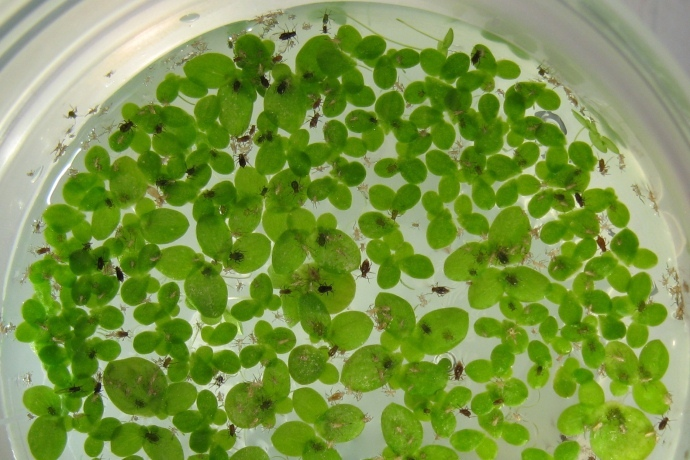
\includegraphics[width=\textwidth]{lemnaspirodellaandaphids.jpg}
\vfill
Modeling of common duckweed and aphid system
\vfill
\end{minipage}%
\pause
\hfill
\begin{minipage}{.48\textwidth}
\vfill
Assuring the safety of UAV operations in close proximity agriculture
\vfill
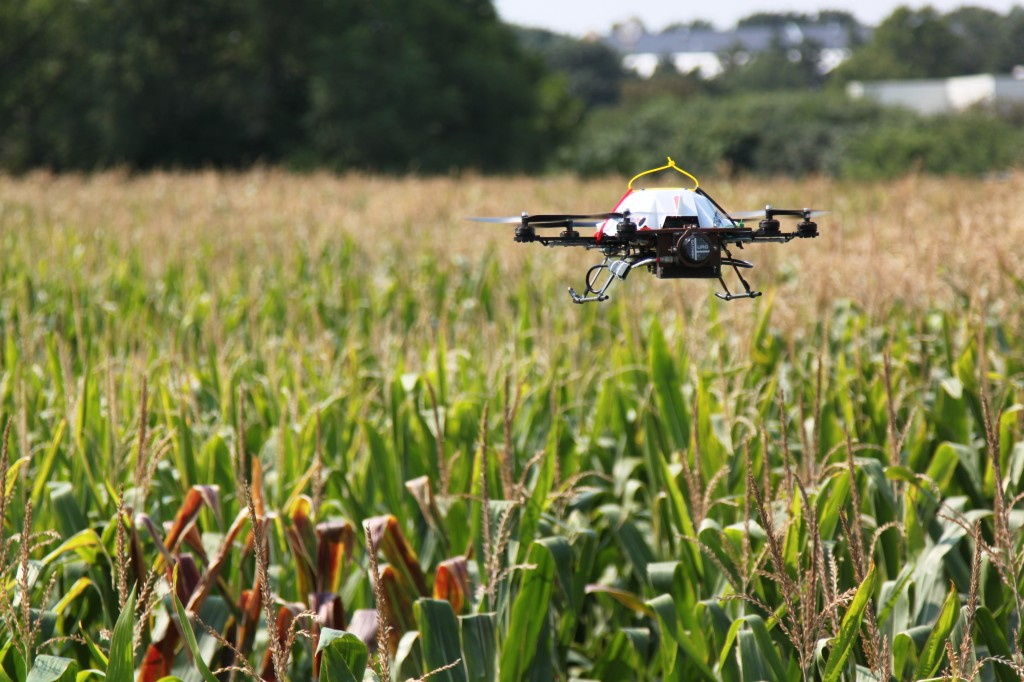
\includegraphics[width=\textwidth]{uav_over_corn-1024x682.jpg}
\vfill
\end{minipage}
\pause
\vfill
\mbox{~}\\
\mbox{~}\\
These systems involve inherent \textbf{uncertainty}
\begin{itemize}
\item in the input values, sensor error, state transitions, ...
\end{itemize}
\vfill
Unlike in classic program analyses, this uncertainty can be characterized and should be exploited 
\vfill
\end{frame}

\begin{frame}[fragile]
\frametitle{What kinds of questions can you answer?}
\vfill
How reliable is the program under an input distribution?
\vfill
How frequently is this block executed?
\vfill
Are these programs equivalent under an input distribution?
\vfill
How sensitive is a test oracle to input distribution?
\vfill
How much of the input space is covered?
\vfill
How important is this dependence? (quantified info. flow)
\vfill
If you can't prove it, how close did you get?
\vfill
\end{frame}

\begin{frame}[fragile]
\frametitle{What's next ...}
\vfill
\begin{itemize}
\item \textcolor{red}{Provide an overview of the key concepts in data flow analysis and symbolic execution}
\item \textcolor{red}{Describe how researchers have enriched those frameworks with probabilistic reasoning (of varying sorts)}
\item \textcolor{red}{Break down the literature across 3 orthogonal dimensions}
\item Talk in more detail about probabilistic symbolic execution 
\item Give you a list of 5+ PhD topics in this area
\end{itemize}
\vfill
\end{frame}

\end{document}
